\documentclass[11pt]{article}
\usepackage[margin=1in]{geometry}
\usepackage{amsmath,amssymb,amsthm,bm}
\usepackage{graphicx}
\usepackage{booktabs}
\usepackage[numbers,sort&compress]{natbib}
\usepackage{hyperref}
\usepackage{xcolor}
\newtheorem{proposition}{Proposition}
\newtheorem{remark}{Remark}
\newcommand{\E}{\mathbb{E}}
\newcommand{\R}{\mathbb{R}}
\newcommand{\sg}{\sigma}
\newcommand{\todo}[1]{\textcolor{red}{[#1]}}

\title{Context length and readout parameterisation select the emergence exponent\\ of in-context skills in an additive model}
\author{\todo{authors}}
\date{Draft v0.2 --- \today}

\begin{document}
\maketitle

\begin{abstract}
We study how a feature-learning model acquires \emph{skills} that are presented in context. Targets are additive models
$y=\sum_p c_p\,\sg(\langle v_p,x\rangle)$ with mean-zero task coefficients $c_p$, and a student with learned features and a
linear-in-label attention readout must recover the directions $v_p$ by online SGD from prompts of length $N$. For a single
skill of information exponent $k^*$ we obtain the population loss in closed form and derive three consequences. (i)~The
in-context loss is the in-weight loss with the link squared, so the effective information exponent is $2k^*$---a fact implicit
in one-step analyses of pretraining, which we make dynamical and test by online SGD. (ii)~A finite context adds an
\emph{alignment-dependent} variance term that makes the unaligned state drift-stable below $m^*\approx\sqrt{2\Gamma/N}$; as a
result, the number of prompts cannot substitute for context length, in contrast to the $N\!\cdot\!T$ trade-off of one-step
analyses. (iii)~A trainable scalar readout relaxes to a Wiener shrinkage factor that starves feature learning and raises the
effective exponent towards $4k^*$ as $N$ decreases, whereas a readout tied to the feature norm does not. A parameter-free
population ODE predicts the SGD-measured exponents across readout protocols and context lengths (12/12 cells within $0.5$).
With many skills of frequencies $\pi_p$ the dynamics decouple with emergence times $\propto 1/\pi_p$---a $1.6$--$2\times$ steeper ordering
by frequency than in-weight learning---and additive compositions of learned skills cost nothing. In small softmax transformers the
effect appears as a $\approx3\times$ per-token handicap of short contexts accompanied by a collapsing readout, not as a trap, and
is invisible when the initial feature alignment is large; we report both regimes.
\end{abstract}

\section{Introduction}
\label{sec:intro}
Theories of feature learning explain \emph{when} a network acquires a direction $v$ in input space in terms of the information
exponent $k^*$ of the link function~\citep{benarous2021online}: online SGD needs $d^{k^*-1}$ samples ($d\log d$ for $k^*=2$). Theories of
emergence and scaling laws~\citep{michaud2023quantization,nam2024exactly,ren2025emergence} then sum many such acquisitions over
a power-law dictionary of skills. Both lines treat the skill as something learned \emph{in the weights} from a fixed task. Large
models, however, acquire much of their behaviour as \emph{in-context} skills: the pretraining data presents a skill through
prompts whose labels are generated by a task-dependent coefficient, and the network must learn features that make the skill
recoverable from a context of length $N$. Recent analyses of in-context learning with learned features~\citep{oko2024pretrained,
nishikawa2025nonlinear,kim2024transformers,gu2026incontext} treat the context length as an \emph{inference-time} resource: it
controls how well a trained model estimates the task, and in one-step analyses of pretraining it enters only through
concentration, so that more prompts can substitute for longer prompts~\citep[Remark~3]{oko2024pretrained}.

We ask a different question: \emph{does the context length, together with how the readout is parameterised, change which
exponent governs the acquisition of a skill during pretraining?} We answer it in the smallest setting in which the question is
sharp---one or several skills with $k^*=2$ (even links, where in-weight learning is easy), a student with features on the sphere
and a linear-in-label readout, online SGD---and then test the predictions outside the solvable model.

\paragraph{Contributions.}
(1)~\textbf{Closed form.} The population in-context loss of a single feature is $L_A(m)=1-2\Gamma g(m)^2+\Gamma^2 g(1)\big[(1-\tfrac1N)g(m)^2+V(m)/N\big]$,
where $m$ is the overlap with the skill direction, $g(m)=\E[\sg(\langle v,x\rangle)\sg(\langle w,x\rangle)]$ and $V(m)=\E[\sg^2\sg^2]$ (Prop.~\ref{prop:loss}).
As $N\to\infty$ it is the in-weight loss with $g\mapsto g^2$: the effective exponent is $2k^*$. The $m^{2k^*-1}$ gradient is
present inside the one-step analysis of \citet[Lemma~21]{oko2024pretrained}; we make the statement dynamical and verify it by
online SGD, including the $k^*=2$ case excluded from \citet{ren2025emergence}.
(2)~\textbf{Finite context creates a drift-stable unaligned state} (Prop.~\ref{prop:repulsion}): the term $\Gamma^2V(m)/N$ grows with
alignment, so for $k^*\ge2$ the origin is stable below $m^{*}$ with $m^{*2}=16\Gamma/\big(N(8-4\Gamma(1-\tfrac1N)-24\Gamma/N)\big)$. Under SGD
the threshold is soft (noise-activated escape), and increasing the number of prompts per step does not remove it (Fig.~\ref{fig:threshold}).
(3)~\textbf{The readout parameterisation selects the exponent} (Prop.~\ref{prop:shrink}): a free scalar readout relaxes to the Wiener value
$\Gamma^*(m)=g^2/\big((1-\tfrac1N)g^2+V/N\big)$ and multiplies the feature gradient, giving effective exponent $4k^*$ where the context statistic
is noise-dominated ($d\gg N^{1/k^*}$), while a readout tied to the feature norm has norm-independent directional dynamics and stays at
$2k^*$. The population ODE predicts the SGD exponents measured at $d=32$ for three readout protocols and four context lengths
(Fig.~\ref{fig:kappa}).
(4)~\textbf{Many skills and composition.} With a power-law dictionary the dynamics decouple with $T_p\propto1/\pi_p$ (measured slope
$1.44$--$1.53$ for $\pi_p\propto p^{-1.5}$), $1.6$--$2\times$ the in-weight slope; additive compositions of learned skills emerge with the slower
skill and cost no extra time, product compositions are not learned.
(5)~\textbf{Transformers.} In a two-layer softmax transformer in the small-alignment regime ($d=256$, width 32) a context of 16
with $16\times$ the prompts emerges $\approx3\times$ later than a context of 256 at equal tokens per step, and the readout norm collapses
while the skill is unlearned; at $d=32$, width 256 (large initial alignment) the ordering reverses. We report both as the boundary of
the mechanism.

\section{Setting}
\label{sec:setup}
Inputs $x\sim\mathcal N(0,I_d)$. A \emph{skill} is a unit vector $v_p\in S^{d-1}$ with link $\sg$; we use the normalised Hermite
polynomials $\sg_k=\mathrm{He}_k/\sqrt{k!}$, so $\E[\sg_j(\langle u,x\rangle)\sg_k(\langle w,x\rangle)]=\delta_{jk}\langle u,w\rangle^k$ for unit
$u,w$ and $k^*=k$. A \emph{task} is a coefficient vector $c$ with independent mean-zero entries, $\E c_p^2=s_p^2$; a \emph{prompt}
consists of $N$ pairs $(x_i,y_i)$ with $y=\sum_p c_p\sg(\langle v_p,x\rangle)$ and a query $(x_q,y_q)$ from the same task. With a
dictionary of $P$ skills and single-skill prompts, skill $p$ appears with frequency $\pi_p$.

\paragraph{Model A (in-context).} Features $\phi_j(x)=\sg(\langle w_j,x\rangle)$, $w_j\in S^{d-1}$, and a linear-in-label readout
\begin{equation}
\hat y_q=\sum_j\Gamma_j\,\phi_j(x_q)\,A_j,\qquad A_j=\frac1N\sum_{i=1}^N y_i\,\phi_j(x_i),
\label{eq:modelA}
\end{equation}
the MLP-plus-linear-attention architecture of \citet{oko2024pretrained}. We consider three readout protocols: \emph{fixed}
$\Gamma_j=\gamma$; \emph{free}, a trainable scalar; and \emph{tied}, $\Gamma_j=\|u_j\|^2$ with $w_j=u_j/\|u_j\|$ (the 2-homogeneous
student of \citet{ren2025emergence}). \textbf{Model B (in-weight)} is ordinary regression $\hat y=\sum_j a_j\phi_j(x)$ on the fixed
task $c\equiv a$. Both are trained by online spherical SGD on the square loss with fresh data at every step.

Write $g(m)=\sum_k\alpha_k^2m^k$ for $\sg=\sum_k\alpha_k\sg_k$ and $V(m)=\E[\sg(\langle v,x\rangle)^2\sg(\langle w,x\rangle)^2]=\sum_j\beta_j^2m^j$
where $\sg^2=\sum_j\beta_j\sg_j$. For $\sg_2$: $g=m^2$, $V=1+8m^2+6m^4$.

\section{A single skill}
\label{sec:single}

\begin{proposition}[Population loss]
\label{prop:loss}
For $P=1$, one feature at overlap $m=\langle w,v\rangle$, readout $\Gamma$ and $\E c^2=s^2$,
\begin{equation}
L_A(m)=s^2\Big[1-2\Gamma g(m)^2+\Gamma^2 g(1)\Big((1-\tfrac1N)g(m)^2+\tfrac{V(m)}{N}\Big)\Big],
\qquad L_B(m)=1-2a\,g(m)+a^2g(1).
\label{eq:LA}
\end{equation}
\end{proposition}
\begin{proof}[Proof sketch]
Conditional on the task, $A=c\,g(m)+\xi/\sqrt N$ with $\E\xi=0$, $\E\xi^2=c^2(V-g^2)$; $x_q$ is independent of the context, and
$\E[\sg(\langle v,x_q\rangle)\sg(\langle w,x_q\rangle)]=g(m)$, $\E[\sg(\langle w,x_q\rangle)^2]=g(1)$. Expanding $\E(y_q-\hat y_q)^2$ gives~\eqref{eq:LA}.
\end{proof}
We verified~\eqref{eq:LA} by comparing the Monte-Carlo drift $-\E[\partial_wL]\cdot v$ with $-\partial_mL_A$ at $m\in\{0.05,0.1,0.2,0.4\}$ for
$k^*\in\{1,2,3\}$: all 24 points agree within $2.3$ s.e.\ and within $3\%$ for $m\ge0.2$ (Appendix).

\paragraph{The link is squared.} As $N\to\infty$, $L_A=L_B[g\mapsto g^2]$. Near $m=0$ the drift is $4\Gamma s^2k^*\alpha_{k^*}^4m^{2k^*-1}$ against
$2ak^*\alpha_{k^*}^2m^{k^*-1}$ for Model B: the label enters the prediction twice---through the context statistic and through the
comparison with $y_q$---and the mean-zero task prior removes the cross terms that would provide a degree-$k^*$ path. (A bias added
to $A_j$ restores an in-weight path of exponent $k^*$ for the \emph{mean} task only; cf.\ \citet{zhang2024incontext} for the linear case.)
With the escape heuristics of \citet{benarous2021online} (drift $\eta Cm^{\kappa-1}$, renormalisation drag $-\eta^2dm/2$) the
timescales are $d^{\kappa-1}$ with $\kappa=2k^*$: for $k^*=2$, in-weight needs $d\log d$ samples and in-context $d^3$.

\begin{proposition}[Finite context: a drift-stable unaligned state]
\label{prop:repulsion}
For $\sg_2$ and fixed readout $\Gamma=\gamma$, $-\partial_mL_A=s^2\big[(8\gamma-4\gamma^2(1-\tfrac1N)-24\gamma^2/N)m^3-16\gamma^2m/N\big]$. The
origin is a local minimum of $L_A$ and the drift is repulsive for $m<m^*$, $m^{*2}=16\gamma/\big(N(8-4\gamma(1-\tfrac1N)-24\gamma/N)\big)\approx2\gamma/(N(1-\gamma/2))$.
\end{proposition}
The variance $V(m)$ of the context statistic \emph{grows} with alignment---an aligned feature has heavy tails that coincide
with the teacher's---so the finite-context noise penalises alignment. A feature initialised at $m_0\approx d^{-1/2}$ is attracted
only if $d\lesssim d^*=N(8-4\gamma(1-\tfrac1N)-24\gamma/N)/(16\gamma)$ ($\approx31$ for $\gamma=1$, $N=128$). For $k^*=1$ the repulsion is a constant
fraction $\gamma/N$ of the attraction and is harmless. One-step analyses of pretraining do not see this term because the readout
is initialised at $\gamma\propto d^{-k^*}$~\citep[Lemma~18]{oko2024pretrained}, which makes $\Gamma^2V/N$ negligible; the phenomenon lives where
$\Gamma$ is order one or trained.

\begin{remark}[Soft under SGD]
SGD is a diffusion on the sphere; a run started below $m^*$ escapes with a Kramers-type probability $\sim e^{-\Delta L/D_{\rm eff}}$,
$\Delta L=L(m^*)-L(m_0)$, $D_{\rm eff}=\eta\,\mathrm{Var}(\partial_m\text{-gradient})/2$. At $\gamma=1$, $N=128$: $d=16$ has $m_0>m^*$ (no barrier),
$d=32$ sits on the ridge ($\Delta L/D_{\rm eff}\approx0.02$), $d=64$ is trapped ($\Delta L/D_{\rm eff}\approx20$). Observed escapes in $3\cdot10^5$ steps: $3/3$, $1/3$, $0/3$.
Larger batches lower $D_{\rm eff}$ and \emph{deepen} the trap.
\end{remark}

\begin{proposition}[Readout parameterisation]
\label{prop:shrink}
(a) \emph{Free readout.} At fixed $m$ the scalar $\Gamma$ relaxes at rate $\approx2V/N$ to
$\Gamma^*(m)=g^2/\big(g(1)[(1-\tfrac1N)g^2+V/N]\big)$, and $L_A(m,\Gamma^*)\approx s^2[1-Ng^4/(g(1)V)]$ for $g^2\ll V/N$, i.e.\ the effective
exponent is $4k^*$ while $m\ll N^{-1/(2k^*)}$ and $2k^*$ beyond. (b) \emph{Tied readout} $\Gamma=\rho=\|u\|^2$: the directional
drift is $(1-m^2)\big[4gg'-\rho(2(1-\tfrac1N)gg'+V'/N)\big]$---the attraction does not carry $\rho$---and $\dot\rho=-4\rho\,\partial_\rho L$ keeps
$\rho$ small; the effective exponent is $2k^*$ for every $N$, while the repulsion of Prop.~\ref{prop:repulsion} survives.
\end{proposition}
The static value $\Gamma^*$ is the ridge/Wiener optimum that appears in replica analyses of trained
models~\citep[eq.~(298)]{gu2026incontext}; our point is its \emph{dynamical} effect: the optimal readout shrinks an untrustworthy
context statistic, and the shrunken readout multiplies the feature gradient, so feature learning is starved exactly when the
context is too short to make the feature useful. That a fast readout doubles the exponent of an in-weight problem is known
\citep[\S5]{bietti2023learning}; what is specific to the in-context problem is that the finite-context noise makes the readout
fast, pins it at $\Gamma^*$, and makes the outcome depend on whether the readout can shrink independently of the feature norm.

\paragraph{Experiment 1 (exponents by SGD).}
Online SGD, $\sg_2$, $d=32$, $\eta=1/d^2$, initial overlap $m_0=c\,d^{-1/2}$, $c\in\{0.5,0.7,1,1.4\}$, three seeds each; the escape
time from $m_0$ scales as $m_0^{-(\kappa-2)}$ for $\kappa>2$, so the slope of $\log T_{0.5}$ against $\log m_0$ measures $\kappa_{\rm eff}=2-\text{slope}$.
Fig.~\ref{fig:kappa} shows $\kappa_{\rm eff}$ for free ($\eta_\Gamma=\eta$ and $10\eta$) and tied readouts at $N\in\{32,128,512,4096\}$ against the
population ODE of Props.~\ref{prop:loss}--\ref{prop:shrink} evaluated at the same $d$, $m_0$-grid, $\Gamma_0$ and $\eta_\Gamma/\eta$: tied
$4.10$--$4.44$ (ODE $4.15$--$4.18$); free $4.8$--$6.6$ rising as $N$ falls (ODE $4.85$--$7.0$); every cell within $\approx0.2$--$0.5$, the $N=32$
cells biased low by censoring. The in-weight model at the same $k^*$ gives a logarithmic $m_0$-dependence ($\kappa=2$). The
pre-registered asymptotes $4\to8$ are the $d\to\infty$ limits; at $d=32$ the same ODE predicts $4.85\to7.0$, which is what SGD shows.

\begin{figure}[t]
\centering
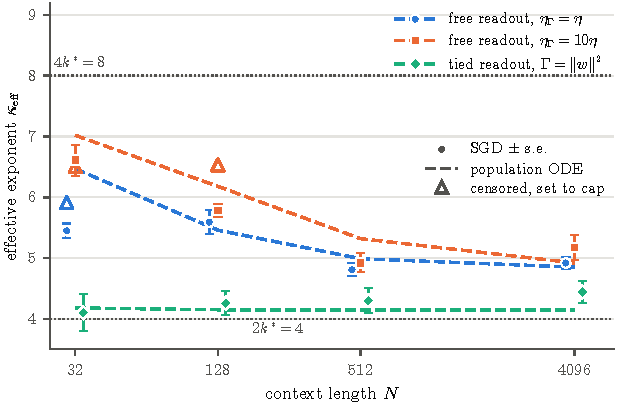
\includegraphics[width=.63\linewidth]{figs/fig_kappa.pdf}
\caption{Effective exponent of skill acquisition for $k^*=2$ at $d=32$: online SGD (points, $\pm$s.e.; triangles: censored runs
set to the step cap) against the parameter-free population ODE (dashed). The tied readout stays at $2k^*=4$; the free readout
rises towards $4k^*=8$ as the context shortens.}
\label{fig:kappa}
\end{figure}

\begin{figure}[t]
\centering
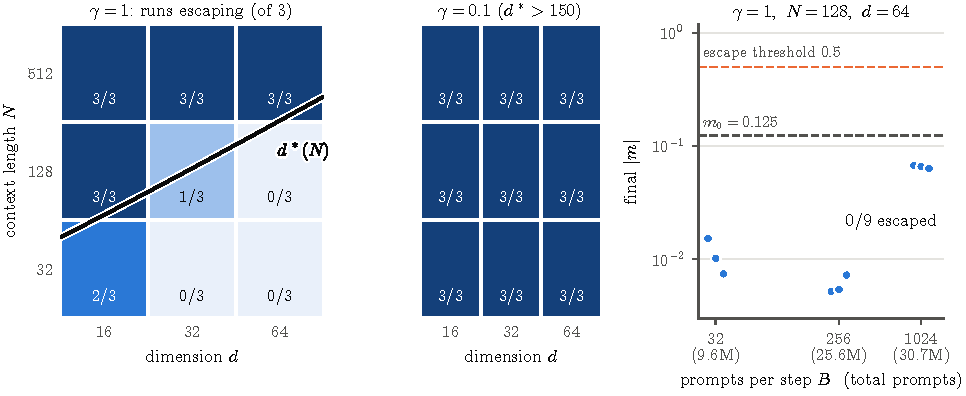
\includegraphics[width=\linewidth]{figs/fig_threshold.pdf}
\caption{Left: fraction of runs escaping $m_0=d^{-1/2}$ within $3\cdot10^5$ steps (fixed readout, 3 seeds per cell; curve: $d^*(N)$ of
Prop.~\ref{prop:repulsion}; for $\gamma=0.1$ the curve lies above the grid). Right: at $\gamma=1$, $N=128$, $d=64$ no run escapes for
$B\in\{32,256,1024\}$ prompts per step (total prompts $\times1$, $\times2.7$, $\times3.2$) and the final overlap falls \emph{below} $m_0$:
more prompts do not substitute for context length.}
\label{fig:threshold}
\end{figure}

\section{Many skills and composition}
\label{sec:many}
Fig.~\ref{fig:many} summarises Exps.~2--3. With $P$ orthogonal skills and $M\ge P$ features the loss splits, when each feature is assigned to one skill, into
$\sum_p\pi_p s_p^2\,\ell(m_p)$ with $\ell$ the single-skill loss; each overlap then follows the single-feature dynamics with rate
$\propto\pi_ps_p^2\Gamma$, so $T_p\propto1/\pi_p$. In-weight learning of the same dictionary carries the coefficient $a_p$ (with
$a_p^2\propto\pi_p$), hence $T_p\propto1/a_p\propto\pi_p^{-1/2}$: \emph{in-context learning orders skills by frequency about twice as steeply} (measured $1.6$--$2\times$).
\textbf{Experiment 2} ($d=32$, $P=16$, $\pi_p\propto p^{-1.5}$, $M=64$, fixed $\Gamma=0.1$, three seeds) gives slopes of $\log T_p$ versus $\log p$ of
$1.44\pm0.08$ (drop midpoints; $1.53\pm0.22$ with the $0.5$-crossing) for the in-context model, against $0.75\pm0.08$ for a capacity-matched in-weight baseline and $0.75$--$0.89$ for the
2-homogeneous in-weight student of \citet{ren2025emergence} (small initialisation, no hand-chosen readout; the lower value is
limited by the logging resolution, the higher one uses a dense early log). Both in-weight baselines fit the target
\emph{collectively} at $M=64>d$ (every skill shared by $\ge2$ features, pooled alignment $\to1$, no single feature above $0.9$), so the
in-weight slope is an empirical baseline rather than a decoupled-neuron prediction; its emergence times nonetheless obey
$T_p\,\eta\,a_p=\mathrm{const}$ ($0.23$--$0.26$ across skills and three learning rates), i.e.\ ordering by the coefficient $a_p\propto\sqrt{\pi_p}$,
whereas the in-context times obey $T_p\,\eta\,\pi_p m_0^2=\mathrm{const}$. The
constant $T_{p}\,\eta\,\pi_p m_0^2=0.73$ (IQR $0.70$--$0.77$) across skills and seeds equals the single-feature value ($0.64$), i.e.\ the
many-skill dynamics is the single-feature dynamics with rate $\pi_p$. Per-skill drops are $\approx4\times$ sharper than in-weight
(relative width $1.08$ vs $4.09$). The frequency-weighted alignment loss decays as $t^{-0.40\pm0.04}$ over the window in which skills
3--8 emerge, against $(\alpha-1)/\alpha=0.33$ for an idealised staircase; the window spans only a factor 3--8 in time, so the exponent
depends on the emergence definition and we do not claim a scaling-law ratio.

\paragraph{Composition.} Because~\eqref{eq:modelA} is linear in the context labels, $\hat y_q(c_1,c_2)=\hat y_q(c_1,0)+\hat y_q(0,c_2)$
identically, and for independent mean-zero $c_1,c_2$ the loss on an additive pair is the sum of the single-skill losses. Trained on
single-skill prompts only ($d=32$, $P=2$, $\pi=0.75/0.25$, $M=4$), the pair loss reaches $90\%$ of its drop before or together with the
slower skill in every run (never after), in contrast to the extra delay for tuples predicted by \citet{arora2023theory}; the
thresholded pair accuracy is approximately the product of the single-skill accuracies ($\mathrm{acc}_{12}\approx0.85\,\mathrm{acc}_1\mathrm{acc}_2+0.09$, r.m.s.\
$0.008$ from $y=x$)---the multiplicative emergence observed empirically by \citet{okawa2023compositional}---while a Gaussian-error
closed form fails (heavy tails). A product composition $\sg_1(\langle v_1,x\rangle)\sg_1(\langle v_2,x\rangle)$ is never learned (loss $\approx1$).

\begin{figure}[t]
\centering
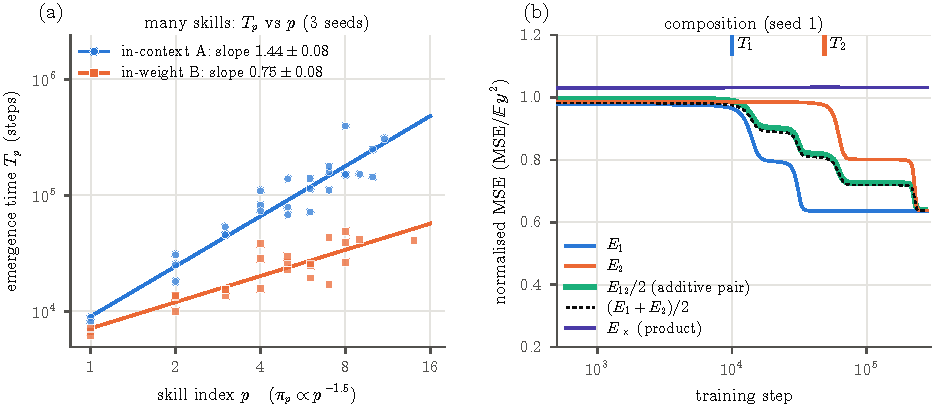
\includegraphics[width=\linewidth]{figs/fig_many.pdf}
\caption{(a) Emergence time (drop midpoint) of skill $p$ versus skill index for the in-context model (slope $1.44\pm0.08$), the
capacity-matched in-weight baseline (slope $0.75\pm0.08$) and the 2-homogeneous in-weight student (slope $0.75$--$0.89$), $\pi_p\propto p^{-1.5}$,
three seeds each; unlearned skills omitted.
(b) Composition (Exp.~3, one seed): normalised MSE on skill-1 prompts, skill-2 prompts, the additive pair (halved) and the product
pair; the dotted curve is half the sum of the single-skill losses and lies on the pair curve. Plateaus at $0.64$ are the fixed-readout
floor $(1-\Gamma n)^2$, not zero.}
\label{fig:many}
\end{figure}

\begin{figure}[t]
\centering
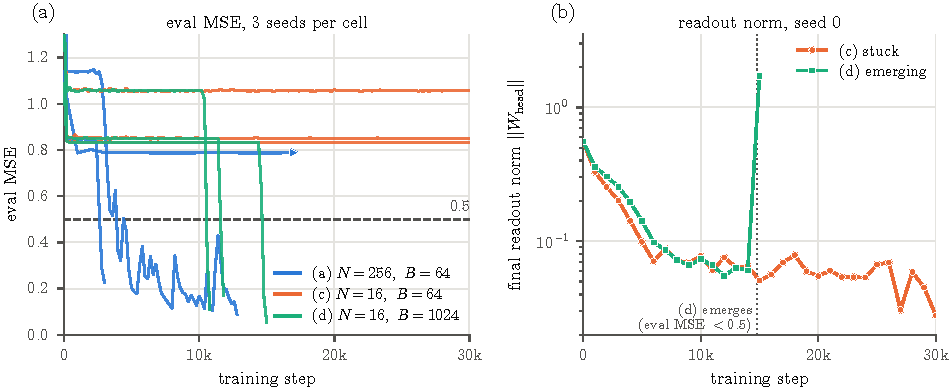
\includegraphics[width=\linewidth]{figs/fig_transformer.pdf}
\caption{Two-layer softmax transformer, $d=256$, MLP width 32, $k^*=2$. (a) Evaluation MSE for $N{=}256,B{=}64$; $N{=}16,B{=}64$; and
$N{=}16,B{=}1024$ (same tokens per step as the first), three seeds each; one $N{=}256$ seed was censored at $17$k steps on the plateau.
(b) Norm of the final readout for one stuck run ($N{=}16,B{=}64$) and one emerging run ($N{=}16,B{=}1024$, same seed): the norm
collapses while the skill is unlearned; the regrowth at emergence is a single logged point (norms logged every $1000$ steps).}
\label{fig:transformer}
\end{figure}

\section{Transformers: where the effect shows and where it does not}
\label{sec:transformer}
We train two-layer softmax transformers (4 heads, pre-LN, Adam, online data; Fig.~\ref{fig:transformer}) on the same in-context task with $k^*=2$ and ask
whether a short context can be compensated by more prompts per step. \textbf{Large initial alignment} ($d=32$, MLP width 256; the best
of 256 random first-layer directions already has $|\cos|=0.43$--$0.55$ with $v$): at a fixed $8192$ tokens per step the emergence step
\emph{increases} with $N$ ($1000/1400/2800$ for $N=16/64/256$)---fewer prompts per step dominate and the mechanism is invisible, as it
must be when $m_0\gg m^*$. \textbf{Small initial alignment} ($d=256$, width 32; $|\cos|_0=0.13$--$0.18$): $N=16$ with $B=64$ prompts never
emerges in $30$k steps ($3/3$); $N=16$ with $B=1024$ (the same tokens per step as $N=256$, $B=64$) emerges in all seeds but at
$10.6$--$14.8$k steps, $\approx3\times$ later than $N=256$ ($2.8$--$4.0$k); while a run is stuck its final readout norm collapses from $0.57$ to
$0.03$--$0.16$, and the first norm logged after emergence is back at $1.7$. Neither pre-registered extreme (a trap, or interchangeability of $N$ and $B$) holds: in the
transformer, context tokens are worth $\approx3\times$ more than prompt tokens for acquiring an even skill, and the readout shrinks
while the skill is unlearned. We state this as an observation consistent with---not a confirmation of---the mechanism of
Sec.~\ref{sec:single}; $k^*=1$ and in-weight controls emerge within $1.4$k and $0.4$k steps.

\section{Related work}
\label{sec:related}
\citet{oko2024pretrained} analyse the architecture~\eqref{eq:modelA} with one gradient step; the product of two correlations
($\propto m^{2Q-1}$) is in their Lemma~21 and the exponent $2Q$ in their total sample count $N_1T_1=\tilde\Omega(d^{2Q+1}r)$, framed as a
consequence of correlational information; their Remark~3 states the $N_1$--$T_1$ trade-off that Prop.~\ref{prop:repulsion} and
Fig.~\ref{fig:threshold} contradict beyond the one-step regime. \citet{nishikawa2025nonlinear} show that softmax's label
nonlinearity lowers the \emph{inference-time} context length to the generative exponent while one-step pretraining stays at
$d^{\Theta(\mathrm{ie})}$. \citet{gu2026incontext} derive, by the replica method for trained models with $k^*=1$, the kernel-vs-feature
context-length scalings and the static shrinkage $\Gamma^*$; they list jointly trained readouts and $k^*\ge2$ as open, which is where our
results sit. \citet{kim2024transformers} note that at finite sample size the ICL landscape may acquire a spurious minimum at the
origin (their App.~C.4), a qualitative precursor of Prop.~\ref{prop:repulsion}. \citet{ren2025emergence} treat the additive model
in-weight for even links with $k^*>2$ with a 2-homogeneous student; our tied protocol is theirs, and $k^*=2$ is outside their
assumptions. The doubling of the exponent by a fast link is in \citet[\S5]{bietti2023learning} and \citet{bietti2022learning}.
\citet{zhang2024incontext} prove, for linear regression, that the task mean is learned in-weight by the MLP and the covariance
in-context. Skill-based accounts of emergence~\citep{michaud2023quantization,nam2024exactly,arora2023theory,okawa2023compositional}
are in-weight; our composition result is the label-linear in-context counterpart. Compositions that are not output-additive need
extra structure~\citep{kobayashi2024compositional,wang2026power,he2024learning}.

\section{Limitations}
\label{sec:limits}
The theory is for one feature per skill and $k^*=2$; the SGD threshold is soft; the many-skill statements rest on decoupling,
which fails for rare skills when no feature starts closest to them (2/10 seeds in Exp.~3); the Gaussian closed form for
compositional accuracy is wrong; the transformer results are observational and were pre-registered with predictions that failed in
both directions. All predictions, outcomes and deviations (including two algebra slips corrected after pre-registration and two
ill-posed estimators) are listed verbatim in the appendix.

\paragraph{Reproducibility and disclosure.} Code, pre-registration document and all runs: \todo{repo}. AI assistance was used for
literature search, implementation, derivation checking and drafting; every derivation was verified against the Monte-Carlo drift,
and every citation against the full text.

\bibliographystyle{plainnat}
\bibliography{refs}
\appendix
\section{Derivations}
\label{app:deriv}

\paragraph{Hermite algebra.} For unit $u,w$ with $\langle u,w\rangle=m$ and $z_u=\langle u,x\rangle$, $z_w=\langle w,x\rangle$ jointly Gaussian with
correlation $m$, $\E[\sg_j(z_u)\sg_k(z_w)]=\delta_{jk}m^k$. For $\sg=\sg_2=(z^2-1)/\sqrt2$: $\sg_2^2=\sqrt6\,\sg_4+2\sqrt2\,\sg_2+1$, hence
$V(m)=\E[\sg_2(z_u)^2\sg_2(z_w)^2]=6m^4+8m^2+1$ and $g(m)=m^2$. For $\sg_1=z$: $g=m$, $V=1+2m^2$.

\paragraph{Population loss (Prop.~\ref{prop:loss}).} With $A=\frac1N\sum_iy_i\sg(\langle w,x_i\rangle)$ and $y_i=c\,\sg(\langle v,x_i\rangle)$,
$\E[A\mid c]=c\,g(m)$ and $\mathrm{Var}[A\mid c]=c^2(V(m)-g(m)^2)/N$. Since $x_q$ is independent of the context,
$\E[y_q\hat y_q]=\Gamma\,\E c^2\,g(m)^2$ and $\E[\hat y_q^2]=\Gamma^2g(1)\,\E c^2\,\big(g^2+(V-g^2)/N\big)$, giving~\eqref{eq:LA}.

\paragraph{Drift (Prop.~\ref{prop:repulsion}).} For $\sg_2$, $\Gamma=\gamma$, $s^2=1$:
$L_A=1-2\gamma m^4+\gamma^2\big[(1-\tfrac1N)m^4+(1+8m^2+6m^4)/N\big]$, so
$-\partial_mL_A=\big(8\gamma-4\gamma^2(1-\tfrac1N)-24\gamma^2/N\big)m^3-16\gamma^2m/N$, which is negative for $m<m^*$ with
$m^{*2}=16\gamma/\big(N(8-4\gamma(1-\tfrac1N)-24\gamma/N)\big)$. (An earlier draft of this derivation dropped the $24\gamma^2/N$ term and
had a factor 2 in the cubic coefficient; the closed-form loss, which the Monte-Carlo drift check verifies directly, was unaffected.)

\paragraph{Population ODEs (Prop.~\ref{prop:shrink}).} Spherical gradient flow for the overlap and plain flow for the readout:
free readout $\dot m=-(1-m^2)\partial_mL_A$, $\dot\Gamma=-r\,\partial_\Gamma L_A$ with $r=\eta_\Gamma/\eta$; tied readout
$\dot m=(1-m^2)\big[4gg'-\rho(2(1-\tfrac1N)gg'+V'/N)\big]$, $\dot\rho=-4\rho\,\partial_\rho L_A$. The chain rule through $\hat u=u/\|u\|$
gives the directional drift a factor $1/\|u\|$ that cancels the $\rho=\|u\|^2$ in the attraction term but not in the repulsion.
Escape times $T_{0.5}$ to $m=0.5$ from $m_0=c\,d^{-1/2}$ were integrated with an adaptive step ($1\%$ relative change per step) and
the exponent read off as $\kappa_{\rm eff}=2-\partial\log T/\partial\log m_0$ over $c\in\{0.5,0.7,1,1.4\}$, exactly as for the SGD data.

\paragraph{Monte-Carlo drift check.} $d=16$, $N=128$, $\gamma=0.1$, $a=1$, $5\cdot10^4$ batches of $64$ prompts per point.
Ratios MC/formula at $m=0.2$ and $0.4$: Model B $k^*=1,2,3$: $0.998$--$1.00$; Model A $k^*=1$: $1.000$; $k^*=2$: $0.972$, $0.998$;
$k^*=3$: $0.88\pm0.76$ (drift $\approx0$), $1.02$. Model A $k^*=3$ at $\gamma=0.1$, $N=128$ has negative drift for $m\le0.2$.

\section{Experimental details}
\label{app:exp}
All toy experiments: float64 numpy, analytic gradients verified by finite differences (relative error $<10^{-4}$), online spherical
SGD with fresh data each step, $B=32$ prompts per step unless stated, $\eta=\eta_0/d^2$. Projected samplers (exact in distribution)
were used where the gradient depends on $x$ only through a few projections. Compute: Exp.~1 $6.4$, Exp.~1b $2.8$, Exp.~2 $3.2$,
Exp.~3 $2.3$, Exp.~4 $6.0$, Exp.~5 $6.0$ CPU-hours on 4 cores.

\paragraph{Exp.~1 (single skill, uniform initialisation).} $k^*\in\{1,2\}$, $d\in\{8,\dots,128\}$, 5 seeds, $N=128$, fixed $\gamma=0.1$ (A) and
$a=1$ (B). Slopes of $\log T_{0.5}$ vs $\log d$: B $k^*=1$: $1.98\pm0.06$ ($d\ge16$; the pre-registered $1.5$ was an error: for $\kappa<2$ the drift
is $O(1)$ and $T\propto1/\eta=d^2$); B $k^*=2$: $2.33\pm0.22$; A $k^*=1$: $2.71\pm0.43$; A $k^*=2$: $3.1$--$3.5$ (20 of 105 runs censored at
$3\cdot10^6$ steps). Regression of $\log(T_{0.5}\eta)$ on $\log|m_0|$: A $k^*=2$: $-2.19\pm0.08$ ($\kappa\approx4.2$, lower bound because of
censoring); B $k^*=2$: $-0.57\pm0.06$ (logarithmic, $\kappa=2$); A $k^*=1$: $-0.50\pm0.06$; B $k^*=1$: $-0.13\pm0.02$.

\paragraph{Exp.~1b (fixed $m_0$).} Threshold grid: $\gamma\in\{1,0.1\}$, $N\in\{32,128,512\}$, $d\in\{16,32,64\}$, 3 seeds, $3\cdot10^5$ steps.
Escapes at $\gamma=1$: $N=32$: $2/3,0/3,0/3$; $N=128$: $3/3,1/3,0/3$; $N=512$: $3/3,3/3,3/3$ (corrected $d^*=6.8,\,30.8,\,126.8$).
$\gamma=0.1$: $27/27$. P7: $\gamma=1$, $N=128$, $d=64$, $B\in\{32,256,1024\}$ with $3\cdot10^5,10^5,3\cdot10^4$ steps: $0/9$ escapes, final
$|m|$ $0.005$--$0.015$ ($B\le256$) and $0.063$--$0.067$ ($B=1024$). Exponent table ($d=32$, 4 values of $m_0$, 3 seeds, $\eta=1/d^2$,
$\Gamma_0=0.01$ or $\rho_0=0.01$): in Fig.~\ref{fig:kappa}; censored runs ($N=32$: 3/12 for both free protocols; $N=128$, $10\eta$: 2/12) are
all at the smallest $m_0$.

\paragraph{Exp.~2 (many skills).} $P=16$, $\pi_p\propto p^{-1.5}$, $M=64$, $\Gamma=0.1$, $N=128$, 3 seeds (plus 2 extra and $\alpha=1$).
Skills 1--8 learned in every run; emergence of skills 9--16 partial. In-weight baseline: readout $\rho=\sum_pa_p/M$ (the readout-1
baseline does not learn), collective fit. Slopes and exponents as in Sec.~\ref{sec:many}; the $\alpha=1$ slope is $0.88\pm0.09$ (A) vs
$0.61\pm0.08$ (B).

\paragraph{Exp.~3 (composition).} $P=2$, $\pi=(0.75,0.25)$, $M=4$, $\Gamma=0.1$, $N=128$, 5 pre-registered seeds + 5 extra + 3 at $\Gamma=0.3$.
Additivity residual with a paired estimator (same inputs, 17 queries per context): $\max|R|\le0.0086$ over 13 runs (the pre-registered
independent-set estimator was too noisy, $0.04$--$0.35$). Final neuron assignments (skill~1, skill~2): $(4,0),(2,2),(2,2),(2,1),(2,2)$ for
the pre-registered seeds. Neuron arrival times $T\approx K/(\eta\pi_pm_0^2)$ with $K=0.60$ ($0.54$--$0.78$).

\paragraph{Exps.~4--5 (transformers).} Tokens $[x_i;y_i]$, query $[x_q;0]$; embedding $\mathrm{Linear}(d{+}1\to64)$, 2 pre-LN blocks
(4-head causal softmax attention + ReLU MLP), linear readout; Adam $10^{-3}$, fp32, online data, eval every 200 steps on 2048 held-out
prompts, $T_e$ = first eval with normalised MSE $<0.5$. Exp.~4: MLP width 256, $d\in\{16,32\}$, $N\cdot B=8192$. Exp.~5: $d=256$, width 32,
cells (a) $N{=}256,B{=}64$: $T_e=4000,2800$, third seed censored at $17$k on the plateau; (c) $N{=}16,B{=}64$: none in $30$k ($3/3$); (d)
$N{=}16,B{=}1024$: $14800,10600,11600$; (e) $k^*=1$, $N{=}16,B{=}64$: $1400,1200$; (f) in-weight: $400,200$; initial $\max_j|\cos(W_j,v)|$:
$0.126,0.152,0.176$.

\section{Pre-registration summary}
\label{app:prereg}
All predictions were written to a version-controlled document before the corresponding run; the full text with timestamps,
outcomes and changelog is in the repository (\texttt{docs/preregistration.md}). Summary:

\begin{center}\small
\begin{tabular}{llp{5.6cm}}
\toprule
ID & prediction & outcome \\
\midrule
P1 & MC drift of A, $k^*{=}2$, $\propto m^3$; closed form within 20\% & met (slope $3.14\pm0.07$; $\le3\%$ at $m\ge0.2$) \\
P2 & $\gamma{=}1$, $N{=}128$: stuck for $d\ge32$ & partly ($d{=}64$ stuck, $d{=}32$: 1/3 escaped); threshold formula later corrected, $d^*\approx31$ \\
P3 & $\gamma{=}0.1$: escapes at all $d$ & met (27/27) \\
P4 & free readout: $\kappa$ rises as $N$ falls, $4\to8$ & direction met; magnitudes match the ODE at $d{=}32$ ($4.85\to7.0$), not the asymptotes \\
P4$'$ & tied readout: $\kappa\approx4$ at all $N$ & met ($4.10$--$4.44$) \\
P5 & learned $\Gamma\approx\Gamma^*(0.5;N)$ & not met (relaxation too slow at $\eta_\Gamma=\eta$) \\
P6 & A vs B slope difference $\approx1$ at $k^*{=}2$ & met via $m_0$-regression ($\kappa$ $4.2$ vs $2$); $d$-slopes $0.9\pm0.5$ \\
P7 & no escape at any $B$ & met (0/9) \\
P8 & transformer, $d{=}32$: $T_e$ falls $\ge3\times$ from $N{=}16$ to $256$ at fixed tokens & \textbf{failed, reversed} ($1000\to2800$) \\
P9 & $k^*{=}1$ weak $N$-dependence; in-weight fastest & partly ($\times2.0$; in-weight fastest) \\
P10 & $N$-dependence in both softmax and linear attention & met (same direction) \\
P11a--b & $d{=}256$, width 32: (c) stuck, (d) stuck & (c) stuck 3/3; (d) emerged 3/3 at $\approx3\times$ (a): \textbf{both rival and default failed} \\
P11c & $k^*{=}1$ and in-weight controls fast & met \\
P12 & additivity residual $|R|\le0.02$ & failed as pre-registered (estimator noise); identity confirmed with a paired estimator \\
P13 & no extra compositional delay & supported with substitute statistic (floor made the original unreachable) \\
P14 & multiplicative accuracy, Gaussian closed form & approximately multiplicative; Gaussian form wrong \\
P15 & product composition not learned & met \\
P16 & $T_p$ slopes $1.5$ (A), $0.75$ (B) & met ($1.44$--$1.53$; $0.75$ with capacity-matched B) \\
P17 & A steps $\ge2\times$ sharper & met ($3.8\times$) \\
P18 & loss exponents $0.33$ (A), $0.67$ (B) & A within tolerance ($0.40$); B failed (collective fit saturates) \\
\bottomrule
\end{tabular}
\end{center}

\end{document}
